\documentclass[tikz,border=10pt]{standalone}
\usetikzlibrary{calc}
\usetikzlibrary{angles,quotes,calc}
\usepackage{tkz-euclide} %for right angle marker

\begin{document}
%Q4 i
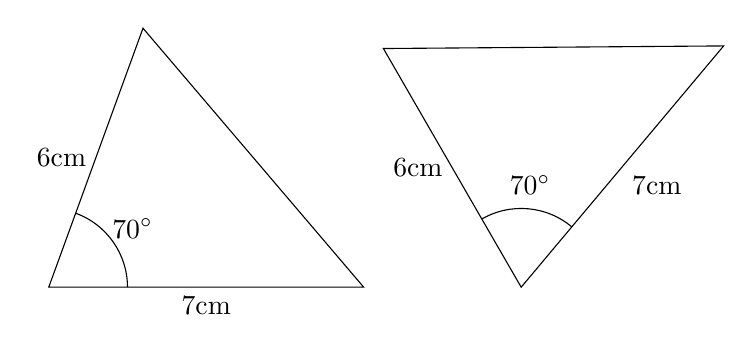
\begin{tikzpicture}
    % Define the first triangle
    \coordinate (A) at (0,0);
    \coordinate (B) at (4,0);
    \coordinate (C) at ($(A)!3.5cm!70:(B)$);

    % Draw the first triangle
    \draw (A) -- node[below]{7cm} (B) -- (C) -- node[left]{6cm} cycle;
    \draw pic["$70^\circ$", draw, angle eccentricity=1.3, angle radius=1cm] {angle=B--A--C};

    % Shift and rotate the first triangle to create the second
    \begin{scope}[shift={(6cm, 0cm)}, rotate=50]
        % Define the 2nd triangle
        \coordinate (D) at (0,0);
        \coordinate (E) at (4,0);
        \coordinate (F) at ($(D)!3.5cm!70:(E)$);

        % Draw the second triangle with the same labels
        \draw (D) -- node[below right]{7cm} (E) -- (F) -- node[left]{6cm} cycle;
        \draw pic["$70^\circ$", draw, angle eccentricity=1.3, angle radius=1cm] {angle=E--D--F};
    \end{scope}
    
\end{tikzpicture}

%Q4 ii
\begin{tikzpicture}
    % Define the first triangle
    \coordinate (A) at (0,0);
    \coordinate (B) at (2,1); % base 4cm
    % Calculate the third point. Adjust the angle if necessary to fit the side lengths.
    \coordinate (C) at ($(A)!3.5cm!75:(B)$); % Adjust the angle to fit the side lengths

    % Draw the first triangle
    \draw (A) -- node[below]{4cm} (B) -- node[above right]{9.5cm} (C) -- node[above left]{7.2cm} cycle;

    % Randomly rotate the first triangle to create the second
    \pgfmathsetmacro{\randomangle}{90} % random angle between -180 and 180 degrees
    \begin{scope}[shift={(8cm, 2cm)}, rotate=\randomangle]
        % Define the second triangle
        \coordinate (D) at (0,0);
        \coordinate (E) at (2,1);
        \coordinate (F) at ($(D)!3.5cm!75:(E)$); % Adjust the angle to fit the side lengths

        % Draw the second triangle with the same labels
        \draw (D) -- node[right]{4cm} (E) -- node[above left]{7.2cm} (F) -- node[below right]{9.5cm} cycle;
    \end{scope}

\end{tikzpicture}

%Q4 iii
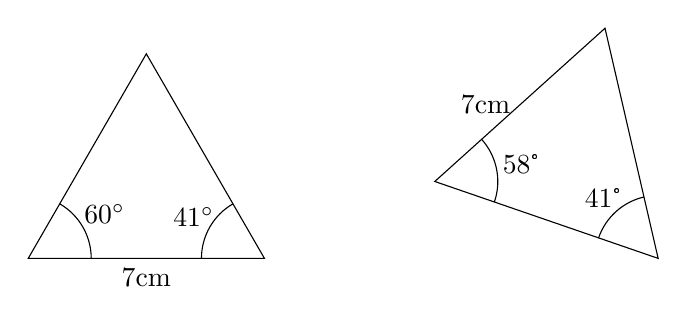
\begin{tikzpicture}
    % Define the first triangle with angles 60 and 41 degrees
    \coordinate[] (A) at (0,0);
    \coordinate[] (B) at (3,0);
    \coordinate[] (C) at ($(A)!3cm!60:(B)$);

    % Draw the first triangle
    \draw (A) -- node[below]{7cm} (B) -- (C) -- cycle;
    \draw pic["$60^\circ$", draw, angle eccentricity=1.4, angle radius=0.8cm] {angle=B--A--C};
    \draw pic["$41^\circ$", draw, angle eccentricity=1.3, angle radius=0.8cm] {angle=C--B--A};

    % Define and draw the second triangle with a different orientation
    \begin{scope}[shift={(8cm, 0)}, rotate=30]
        % Define the second triangle with angles 41 and 58 degrees
        \coordinate[] (D) at (0,0);
        \coordinate[] (E) at ($(D)!3cm!41:(0,1)$);
        \coordinate[] (F) at ($(D)!3cm!-58:(E)$);

        % Draw the second triangle
        \draw (D)   -- (E)  -- node[left]{7cm} (F) -- cycle ;
        \draw pic["41°", draw, angle eccentricity=1.3, angle radius=0.8cm] {angle=F--D--E};
        \draw pic["58°", draw, angle eccentricity=1.4, angle radius=0.8cm] {angle=D--E--F};
    \end{scope}
\end{tikzpicture}

%Q4 iv
\begin{tikzpicture}
    % Define the first right triangle
    \coordinate (A) at (0,0);
    \draw (A) -- ++(180:2cm) coordinate (B) -- ++(90:3cm) coordinate (C) -- cycle; 
    \tkzMarkRightAngle(A,B,C)
    \tkzLabelSegment[below](A,B){3}
    \tkzLabelSegment[above right](A,C){5}

    % Draw the second right triangle, rotated
    \begin{scope}[shift={(4cm, 0cm)}, rotate=-60] % Adjust shift and rotation as needed
       % Define the first right triangle
        \coordinate (A) at (0,0);
        \draw (A) -- ++(180:2cm) coordinate (B) -- ++(90:3cm) coordinate (C) -- cycle; 
        \tkzMarkRightAngle(A,B,C)
        \tkzLabelSegment[below left ](A,B){3}
        \tkzLabelSegment[below right](A,C){5}
    \end{scope}
\end{tikzpicture}

%Q1
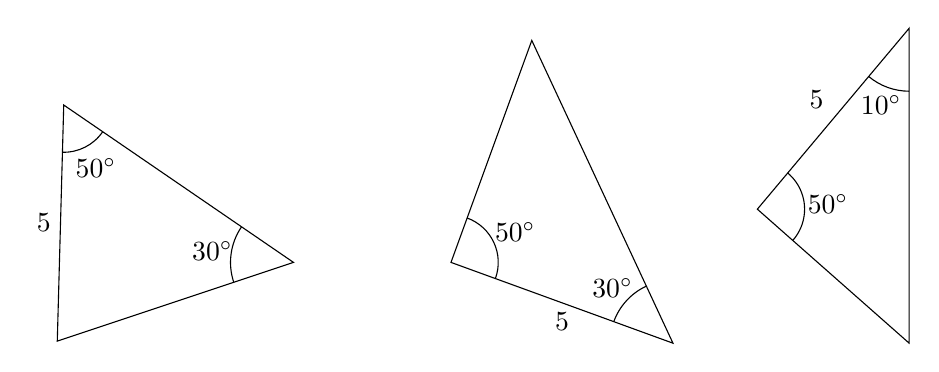
\begin{tikzpicture}
    % First Triangle
    \coordinate (A) at (0,0);
    \coordinate (B) at ($(A)+(3,1)$);
    \coordinate (C) at ($(A)!3cm!70:(B)$);
    \draw (A) -- (B) -- (C) -- cycle;
    \pic [draw, "$50^\circ$", angle eccentricity=1.5, angle radius = 0.6cm] {angle = A--C--B};
    \pic [draw, "$30^\circ$", angle eccentricity=1.3, angle radius = 0.8cm] {angle = C--B--A};
    \tkzLabelSegment[left](A,C){5};

    % Second Triangle (differently oriented)
    \coordinate (D) at ($(B)+(2,0)$); % Shifted to the right
    \coordinate (E) at ($(D)+(70:3cm)$); % Using polar coordinates for a different orientation
    \coordinate (F) at ($(D)!3cm!-90:(E)$);
    \draw (D) -- (E) -- (F) -- cycle;
    \pic [draw, "$50^\circ$", angle eccentricity=1.5, angle radius = 0.6cm] {angle = F--D--E};
    \pic [draw, "$30^\circ$", angle eccentricity=1.3, angle radius = 0.8cm] {angle = E--F--D};
    \tkzLabelSegment[below](D,F){5};
    
    % Third Triangle
    \coordinate (G) at ($(F)+(3,0)$); % Shifted to the right
    \coordinate (H) at ($(G)!4cm!50:(G)$);
    \coordinate (I) at ($(H)!3cm!-40:(G)$);
    \draw (G) -- (H) -- (I) -- cycle;
    \pic [draw, "$50^\circ$", angle eccentricity=1.5, angle radius = 0.6cm] {angle = G--I--H};
    \pic [draw, "$10^\circ$", angle eccentricity=1.3, angle radius = 0.8cm] {angle = I--H--G};
    \tkzLabelSegment[above left](I,H){5};
\end{tikzpicture}

%Q3

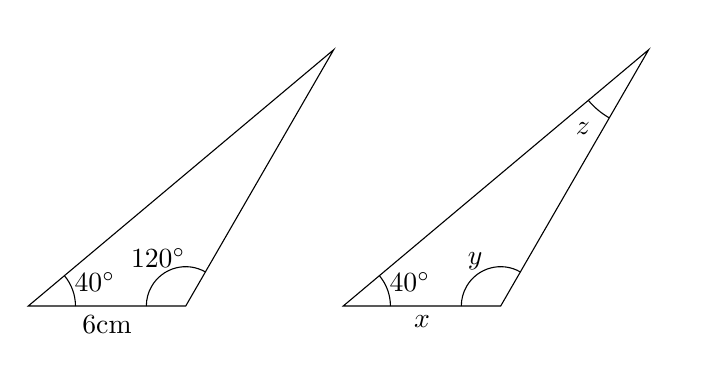
\begin{tikzpicture}
    % First Triangle
    \coordinate (A) at (0,0);
    \coordinate (B) at (2,0); % Base of 3cm

    % Paths at specified angles
    \path[name path=AC] (A) -- ++(40:5.5cm); % Path at an angle 40° from A
    \path[name path=BC] (B) -- ++(60:4cm); % Path at an angle 60° from B (180°-120°)

    % Intersection of paths
    \path[name intersections={of=AC and BC,by=C}];

    % Draw the triangle
    \draw (A) -- (B) -- (C) -- cycle;
    \pic [draw, " $40^\circ$", angle eccentricity=1.5, angle radius = 0.6cm] {angle = B--A--C};
    \pic [draw, " $120^\circ$", angle eccentricity=1.4, angle radius = 0.5cm] {angle = C--B--A};
    \tkzLabelSegment[below](A,B){6cm};

    \begin{scope}[shift={(4cm, 0cm)}]
        \coordinate (A) at (0,0);
        \coordinate (B) at (2,0); % Base of 3cm
    
        % Paths at specified angles
        \path[name path=AC] (A) -- ++(40:5.5cm); % Path at an angle 40° from A
        \path[name path=BC] (B) -- ++(60:4cm); % Path at an angle 60° from B (180°-120°)
    
        % Intersection of paths
        \path[name intersections={of=AC and BC,by=C}];
    
        % Draw the triangle
        \draw (A) -- (B) -- (C) -- cycle;
        \pic [draw, "$40^\circ$", angle eccentricity=1.5, angle radius = 0.6cm] {angle = B--A--C};
        \pic [draw, "$y$", angle eccentricity=1.3, angle radius = 0.5cm] {angle = C--B--A};
        \pic [draw, "$z$", angle eccentricity=1.3, angle radius = 1cm] {angle = A--C--B};
        \tkzLabelSegment[below](A,B){$x$};
    \end{scope}

\end{tikzpicture}

\end{document}
